\chapter{Testy wydajnościowe}
\section{Opis testów}

Do testów przygotowano dwie aplikację. Pierwszą z nich była aplikacja w języku \textsl{Java} uruchomiona na dwóch różnych serwerach: \textsl{Tomcat 8} i \textsl{Jetty 9}. Serwery te są obecnie jednymi z najpopularniejszych rozwiązań służących do uruchamiania aplikacji \textsl{Java}.  Drugą aplikacją była aplikacja w języku \textsl{GO}, która przy użyciu biblioteki \textsl{HttpRouter} (https://github.com/julienschmidt/httprouter) pozwala na tworzenie aplikacji działającej jako serwer \textsl{HTTP}.

Każda aplikacja była testowana przez przygotowany zbiór testów w aplikacji \textsl{Apache JMeter}. \textsl{Apache JMeter} pozwala na tworzenie i wykonywanie testów wydajnościowych, symulujących wielu klientów korzystających z aplikacji. Przygotowane testy zostały podzielone na 4 grupy:
\begin{itemize}
    \item testy sprawdzające wydajność walidacji istnienia klucza \textsl{API}
    \item testy sprawdzające wydajność walidacji obiektu \textsl{Cache}
    \item testy sprawdzające wydajność operacji typu \textsl{CRUD}
    \item testy sprawdzające wydajność powyższych scenariuszy równolegle
\end{itemize}

Pierwsza grupa sprawdzała wydajność aplikacji, gdy klient chciał wykonać operacje posiadając nieistniejący klucz \textsl{API}. Na tą grupę składało się pięć testów, wykonywanej w następującej kolejności:
\begin{enumerate}
    \item pobieranie listy wszyskitch obiektów \textsl{Cache}
    \item pobieranie pojedynczego obiektu \textsl{Cache}
    \item tworzenie obiektu \textsl{Cache}
    \item aktualizacji obiektu \textsl{Cache} 
    \item usunięcie obiektu \textsl{Cache}
\end{enumerate}
Każdy z tych testów oznaczany był jako poprawny, gdy aplikacja zwracała błąd autoryzacji dla każdego żądania.

Drugą grupą testów było sprawdzenie wydajności, gdy klucz \textsl{API} istniał jednak klient chciał przeprowadzić operacje pobierania, usuwania i aktualizacji nie istniejącego obiektu \textsl{Cache}. Scenariusz grupy wyglądał następująco:
\begin{enumerate}
    \item pobierz nowy klucz \textsl{API}
    \item pobierz obiekt \textsl{Cache} autoryzując się otrzymanym kluczem \textsl{API}
    \item zaktualizuj obiekt \textsl{Cache} autoryzując się otrzymanym kluczem \textsl{API}
    \item usuń obiekt \textsl{Cache} autoryzując się otrzymanym kluczem \textsl{API}
\end{enumerate}
Każdy z tych testów oznaczany był jako poprawny, gdy aplikacja zwracała błąd autoryzacji dla każdego żądania.

Kolejną grupą były testy wydajności operacji \textsl{CRUD}. Do przeprowadzenia tej grupy testów został przygotowany zbiór 100 tysięcy losowych wartości w formie pliku \textsl{CSV}. Każda wartość składała się 3 części. Pierwszą był klucz obiektu \textsl{Cache}, natomiast dwie kolejne to wartości, które zostaną zapisane w aplikacji w polu \textsl{value} obiektu. \textsl{Apache JMeter} pozwala na przekazanie pliku \textsl{CSV}, którego wartości można użyć do przeprowadzenia testów. Scenariusz tej grupy wyglądał następująco:
\begin{enumerate}
    \item pobierz nowy klucz \textsl{API}
    \item utwórz obiekt \textsl{Cache} o kluczu i wartości otrzymanym z parametru
    \item pobierz utworzony obiekt \textsl{Cache} 
    \item zaktualizuj obiekt \textsl{Cache} ustawiając nową wartość pola \textsl{value}
    \item usuń obiekt \textsl{Cache}
\end{enumerate}
Każdy z tych testów oznaczany był jako poprawny, gdy aplikacja dla każdego z nich nie zwracała błędu.

Ostatnią grupę stanowiły wszystkie testy, które zostały opisane w powyższych grupach. 

Wszystkie grupy były wykonywane w 15 minutowych cyklach, oddzielonych 60 sekundową przerwą.

Każda aplikacja testowana była w czterech przypadkach testowych. Przypadki te różniły się od siebie liczbą klientów, którzy równolegle wykonywali żądania oraz stanu początkowego bazy danych:
\begin{itemize}
    \item 100 klientów oraz pusta baza danych
    \item 250 klientów oraz pusta baza danych
    \item 100 klientów oraz baza danych wypełniona danymi
    \item 250 klientów oraz baza danych wypełniona danymi
\end{itemize}
W dwóch ostatnich przypadkach baza danych była wypełniona losowymi danymi: 4000000 obiektów w kolekcji \textsl{api}, 40000000 obiektów w kolekcji \textsl{cache}. Łącznie baza danych zajmowała 12 gigabajtów pamięci masowej.

\section{Środowisko testowe}
Do przeprowadzenia testów wydajnościowych wykorzystywane były 3 serwery wirtualne. Specyfikacje techniczne serwerów wirtualnych, wykorzystanych w testach to: 
\begin{itemize}
    \item 8 rdzeni, 16 gigabajtów pamięci RAM, 160 gigabajtów dysku SSD dla serwera aplikacyjnego
    \item 4 rdzenie, 8 gigabajtów pamięci RAM, 80 gigabajtów dysku SSD dla serwera bazy danych 
    \item 4 rdzenie, 8 gigabajtów pamięci RAM, 80 gigabajtów dysku SSD dla serwera, na którym uruchomiony był program \textsl{Apache JMeter}
\end{itemize}
Serwery komunikowały się po sieci lokalnej (ang. \textsl{LAN}) bezpośrednio między sobą.

Na rysunku \ref{fig:deployment_diagram} zaprezentowany został diagram wdrożenia infrastruktury wykorzystanej do przeprowadzenia testów.
\begin{figure}[!ht]
\centering
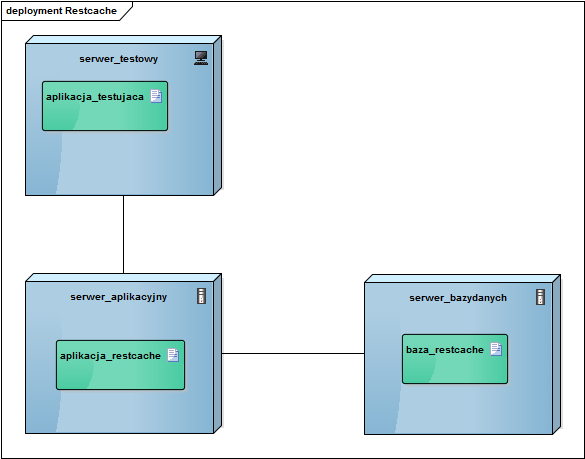
\includegraphics[width=12cm, height=9cm]{\ImgPath/diagram_wdrozenia.png}
\caption{Diagram wdrożenia infrastruktury wykorzystywanej do przeprowadzenia testów}
\label{fig:deployment_diagram}
\end{figure}

\newpage
\section{Wyniki testów - pusta baza danych}

\subsection{Testy wydajności walidacji API}
Pierwszą grupą testów były testy wydajności walidujących istnienie kliczy \textsl{API}. Z diagramów \ref{fig:tomcat_clean_api_validation_rps} i \ref{fig:tomcat_clean_api_validation_td} przedstawiających wydajność aplikacji \textsl{Java} uruchomionej na serwerze \textsl{Tomcat 8} wynika, że przy 100 równolegle uruchomionych klientach liczba obsłużonych żądań wahała się od 6 do 8 tysięcy żądań w ciągu sekundy. Natomiast średni czas odpowiedzi wynosił 11.82 milisekund. W przypadku 250 klientów, którzy testowali aplikację liczba żądań wahała się miedzy 4 a 8 tysiącami, a rozkład czasów odpowiedzi bardzo się spłaszczył. Średni czas odpowiedzi wynosił w tym teście 33.73 milisekundy.

Wyniki testów dla aplikacji \textsl{Java} uruchomionej na serwerze \textsl{Jetty 9} przedstawione są na diagramach \ref{fig:jetty_clean_api_validation_rps} i \ref{fig:jetty_clean_api_validation_td}. W teście przy 100 klientach liczba obsłużonych żądań w ciągu sekundy wahała się od 7 do 10 tysięcy, a średni czas odpowiedzi wyniósł 9.30 milisekund. Na diagramie rozkładu czasów odpowiedzi widać, że największa ilość żądań trwała poniżej 10 milisekund. Dla testu z uruchomionymi 250 klientami liczba żądań wahała się między 5 a 10 tysięcy i rozkład czasów również się spłaszczył. W teście tym średni czas odpowiedzi wyniósł 33.66 milisekund. 

Ostatnią testowaną aplikacją była aplikacja napisana w języku \textsl{Go}. Rozkład liczby żądań obsłużonych w ciągu sekundy (\ref{fig:go_clean_api_validation_rps}) dla testu z wykorzystaniem 100 i 250 klientów jest bardzo zbliżony. Dla 100 klientów oscyluje w okolicy 10 tysięcy żądań, dla 250 klientów w okolicy 9 tysięcy żądań. Analizując rozkład czasów odpowiedzi (\ref{fig:go_clean_api_validation_td}) można zauważyć, że w obu testach jest on symetryczny. Średnie czasy odpowiedzi wyniosły: 8.31 milisekund dla 100 klientów oraz 23.80 milisekund dla 250 klientów.

W tabelach \ref{tab:app-clean-api} oraz \ref{tab:mongo-clean-api} zaprezentowane są średnie wykorzystanie procesora oraz pamięci \textsl{RAM} na maszynach, gdzie uruchomione były aplikacje oraz baza danych \textsl{MongoD}. Aplkacja \textsl{Java} uruchomiona na serwerze \textsl{Tomcat 8} wykorzystywała najbardziej zasoby procesora (77.50\% i 65.73\%), serwer \textsl{Jetty 9} obciążał o około 5\% mniej procesor. Natomiast aplikacja w języku \textsl{Go} wymagała najmniej zasobów procesora (29.93\% i 31.54\%). Serwer \textsl{Jetty 9} potrzebował najwięcej pamięci \textsl{RAM} do działania (ponad 2000 MB), \textsl{Tomcat 8} potrzebował o 100 MB mniej, a aplikacja w języku \textsl{Go} potrzebowała około 210 MB pamięci. Roœnież serwer bazy danych był mniej obciążony w teście aplikacji napisanej w języku \textsl{Go}.

\pgfplotsset{grid style={dashed}}
\begin{figure}[!ht]
\captionsetup[subfigure]{singlelinecheck=off, justification=centering}
\showcaptionsetup{subfigure}
\hspace{-2.5cm}
\begin{subfigure}{0.5\textwidth}
\pgfplotstableread[col sep = comma]{csv_queries/requests_per_sec/tomcat_clean_api_validation.csv}\csvdata
\begin{tikzpicture}
  \begin{axis}[xmin = 0, xmax=900, ymin = 0, scaled y ticks = base 10:-3, xlabel = {Czas [s]}, ylabel = Liczba żądań, legend pos=south east, ymajorgrids] %TODO miary?
    \addplot[color=blue,mark=none] table[x index=0, y index=1]{\csvdata};
    \addplot[color=green,mark=none] table[x index=0, y index=2]{\csvdata};
    \legend{100,250}
  \end{axis}
\end{tikzpicture}
\caption{Tomcat 8 - liczba żądań obsłużonych przez aplikację w ciągu sekundy}
\label{fig:tomcat_clean_api_validation_rps}
\end{subfigure}

\hspace{3cm}
\begin{subfigure}{0.5\textwidth}
\pgfplotstableread[col sep = comma]{csv_queries/response_time_distribution/tomcat_clean_api_validation_100.csv}\csva
\pgfplotstableread[col sep = comma]{csv_queries/response_time_distribution/tomcat_clean_api_validation_250.csv}\csvb
\pgfplotsset{
    /pgfplots/ybar legend/.style={
    /pgfplots/legend image code/.code={\draw[##1,/tikz/.cd,yshift=-0.25em](0cm,0cm) rectangle(1pt,0.7em);},
   }
}
\begin{tikzpicture}
  \begin{axis}[ybar, bar width=0.5, xmin = 0, ymin = 0, scaled y ticks = base 10:-5, xlabel = {Czas odpowiedzi [ms]}, ylabel = {Liczba żądań}, ymajorgrids] %TODO miary?
    \addplot[color=blue, mark=none, fill=blue] table[x index=0, y index=1]{\csva};
    \addplot[color=green, mark=none, fill=green] table[x index=0, y index=1]{\csvb};
    \legend{100,250}
  \end{axis}
\end{tikzpicture}
\caption{Tomcat 8 - rozkład czasów odpowiedzi aplikacji (95\% odpowiedzi)}
\label{fig:tomcat_clean_api_validation_td}
\end{subfigure}

\caption{Tomcat 8 - testy wydajności walidacji istnienia klucza API}
\label{fig:tomcat_clean_api_validation}
\end{figure}

\clearpage
\pgfplotsset{grid style={dashed}}
\begin{figure}[!ht]
\captionsetup[subfigure]{singlelinecheck=off, justification=centering}
\showcaptionsetup{subfigure}
\hspace{-2.5cm}
\begin{subfigure}{0.5\textwidth}
\pgfplotstableread[col sep = comma]{csv_queries/requests_per_sec/jetty_clean_api_validation.csv}\csvdata
\begin{tikzpicture}
  \begin{axis}[xmin = 0, xmax=900, ymin = 0, scaled y ticks = base 10:-3, xlabel = {Czas [s]}, ylabel = Liczba żądań, legend pos=south east, ymajorgrids] %TODO miary?
    \addplot[color=blue,mark=none] table[x index=0, y index=1]{\csvdata};
    \addplot[color=green,mark=none] table[x index=0, y index=2]{\csvdata};
    \legend{100,250}
  \end{axis}
\end{tikzpicture}
\caption{Jetty 9 - liczba żądań obsłużonych przez aplikację w ciągu sekundy}
\label{fig:jetty_clean_api_validation_rps}
\end{subfigure}

\hspace{3cm}
\begin{subfigure}{0.5\textwidth}
\pgfplotstableread[col sep = comma]{csv_queries/response_time_distribution/jetty_clean_api_validation_100.csv}\csva
\pgfplotstableread[col sep = comma]{csv_queries/response_time_distribution/jetty_clean_api_validation_250.csv}\csvb
\pgfplotsset{
    /pgfplots/ybar legend/.style={
    /pgfplots/legend image code/.code={\draw[##1,/tikz/.cd,yshift=-0.25em](0cm,0cm) rectangle(1pt,0.7em);},
   }
}
\begin{tikzpicture}
  \begin{axis}[ybar, bar width=0.5, xmin = 0, ymin = 0, scaled y ticks = base 10:-5, xlabel = {Czas odpowiedzi [ms]}, ylabel = {Liczba żądań}, ymajorgrids] %TODO miary?
    \addplot[color=blue, mark=none, fill=blue] table[x index=0, y index=1]{\csva};
    \addplot[color=green, mark=none, fill=green] table[x index=0, y index=1]{\csvb};
    \legend{100,250}
  \end{axis}
\end{tikzpicture}
\caption{Jetty 9 - rozkład czasów odpowiedzi aplikacji (95\% odpowiedzi)}
\label{fig:jetty_clean_api_validation_td}
\end{subfigure}

\caption{Jetty 9 - testy wydajności walidacji istnienia klucza API}
\label{fig:jetty_clean_api_validation}
\end{figure}

\clearpage
\pgfplotsset{grid style={dashed}}
\begin{figure}[!ht]
\captionsetup[subfigure]{singlelinecheck=off, justification=centering}
\showcaptionsetup{subfigure}
\hspace{-2.5cm}
\begin{subfigure}{0.5\textwidth}
\pgfplotstableread[col sep = comma]{csv_queries/requests_per_sec/go_clean_api_validation.csv}\csvdata
\begin{tikzpicture}
  \begin{axis}[xmin = 0, xmax=900, ymin = 0, scaled y ticks = base 10:-3, xlabel = {Czas [s]}, ylabel = Liczba żądań, legend pos=south east, ymajorgrids] %TODO miary?
    \addplot[color=blue,mark=none] table[x index=0, y index=1]{\csvdata};
    \addplot[color=green,mark=none] table[x index=0, y index=2]{\csvdata};
    \legend{100,250}
  \end{axis}
\end{tikzpicture}
\caption{Go - liczba żądań obsłużonych przez aplikację w ciągu sekundy}
\label{fig:go_clean_api_validation_rps}
\end{subfigure}

\hspace{3cm}
\begin{subfigure}{0.5\textwidth}
\pgfplotstableread[col sep = comma]{csv_queries/response_time_distribution/go_clean_api_validation_100.csv}\csva
\pgfplotstableread[col sep = comma]{csv_queries/response_time_distribution/go_clean_api_validation_250.csv}\csvb
\pgfplotsset{
    /pgfplots/ybar legend/.style={
    /pgfplots/legend image code/.code={\draw[##1,/tikz/.cd,yshift=-0.25em](0cm,0cm) rectangle(1pt,0.7em);},
   }
}
\begin{tikzpicture}
  \begin{axis}[ybar, bar width=0.5, xmin = 0, ymin = 0, scaled y ticks = base 10:-5, xlabel = {Czas odpowiedzi [ms]}, ylabel = {Liczba żądań}, ymajorgrids] %TODO miary?
    \addplot[color=blue, mark=none, fill=blue] table[x index=0, y index=1]{\csva};
    \addplot[color=green, mark=none, fill=green] table[x index=0, y index=1]{\csvb};
    \legend{100,250}
  \end{axis}
\end{tikzpicture}
\caption{Go - rozkład czasów odpowiedzi aplikacji (95\% odpowiedzi)}
\label{fig:go_clean_api_validation_td}
\end{subfigure}

\caption{Go - testy wydajności walidacji istnienia klucza API}
\label{fig:go_clean_api_validation}
\end{figure}

\clearpage


\begin{table}[!htb]
\centering
\caption{Wykorzystanie procesora i pamięci RAM na serwerze, gdzie uruchomiona była aplikacja}
\label{tab:app-clean-api}
\begin{tabular}{@{}ccccl@{}}
\toprule
\textbf{Język} & \textbf{Liczba wątków} & \multicolumn{1}{p{3cm}}{\textbf{Średnie wykorzystanie CPU (\%)}} & \multicolumn{1}{p{3cm}}{\textbf{Średnie wykorzystanie RAM (MB)}} &  \\ \midrule
Tomcat 8       & 100                    & 77.5                             & 1882.6                          &  \\
Tomcat 8       & 250                    & 65.73                             & 1926.08                          &  \\
Jetty 9       & 100                    & 70.13                             & 2020.03                          &  \\
Jetty 9       & 250                    & 59.31                             & 2005.06                          &  \\
Go       & 100                    & 29.93                             & 211.65                          &  \\
Go       & 250                    & 31.64                             & 228.72                          &  \\
\bottomrule
\end{tabular}
\end{table}


\begin{table}[!htb]
\centering
\caption{Wykorzystanie procesora i pamięci RAM na serwerze, gdzie uruchomiona była baza danych MongoDB}
\label{tab:mongo-clean-api}
\begin{tabular}{@{}ccccl@{}}
\toprule
\textbf{Język} & \textbf{Liczba wątków} & \multicolumn{1}{p{3cm}}{\textbf{Średnie wykorzystanie CPU (\%)}} & \multicolumn{1}{p{3cm}}{\textbf{Średnie wykorzystanie RAM (MB)}} &  \\ \midrule
Tomcat 8       & 100                    & 29.4                             & 151.1                          &  \\
Tomcat 8       & 250                    & 22.05                             & 272.9                          &  \\
Jetty 9       & 100                    & 30.29                             & 301.42                          &  \\
Jetty 9       & 250                    & 22.55                             & 270.23                          &  \\
Go       & 100                    & 18.92                             & 302.67                          &  \\
Go       & 250                    & 16.84                             & 358.49                          &  \\
\bottomrule
\end{tabular}
\end{table}


\clearpage

\subsection{Test wydajności walidacji istnienia obiektów Cache}
Kolejną grupą testów były testy wydajności walidacji istnienia obiektów \textsl{Cache}. Diagramy \ref{fig:tomcat_clean_key_validation_rps},  \ref{fig:jetty_clean_key_validation_rps} oraz  \ref{fig:go_clean_key_validation_rps} prezentują rozkład ilości żądań obsługiwanych przez poszczególne aplikacje podczas trwania testu. W przypadku testu z użyciem 100 klientów największą wydajność miała aplikacja napisana w \textsl{Go}. Była ona w stanie obsłużyć ponad 7 tysięcy żądań na sekundę. Serwer \textsl{Jetty 9} z aplikacją \textsl{Java} był w stanie osiągnąć przepustowość od 3.5 do 4.5 tysiąca żądań na sekundę. Najmniejszą przepustowość osiągnął w teście serwer \textsl{Tomcat 8} osiągając wartości między 2.5 a 4 tysiące żądań na sekundę. W przypadku 250 klientów również najlepszy wynik osiągnęła aplikacja w \textsl{Go}. Jej przepustowość była niewiele mniejsza od testu ze stoma klientami. Serwery \textsl{Jetty 9} i \textsl{Tomcat 8} osiągnęły wyniki zbliżone do siebie, odpowiednio: około 3 tysiące i y żądań. Dodatkowo serwer \textsl{Tomcat 8} miał większe wachania przepustowości podczas testu.

Z diagramów rozkładu czasów odpowiedzi (\ref{fig:tomcat_clean_key_validation_td},  \ref{fig:jetty_clean_key_validation_td}, \ref{fig:go_clean_key_validation_td}) wynika, że podczas próby 100 klientów najlepsze wyniki osiągneła aplikacja w \textsl{Go}, gdzie najdłużej trwające żądania trwały 25 milisekund, a średnia wyniosła 12.80 milisekund. Rozkład czasów serwera \textsl{Jetty} był bardzo równy, a średnia czasów odpowiedzi wyniosła 21.55 milisekund. Najdłuższe czasy zanotowano w teście serwera \textsl{Tomcat 8}, gdzie średnia odpowiedzi wyniosła 26.73 milisekundy, jednak najdłuższe żądania trwały 120 milisekund podczas testu. W teście z 250 klientami również najmniejsza średnia jest w aplikacji napisanej w \textsl{Go} (30.43 milisekundy). Następny był serwer \textsl{Jetty 9} ze średnią 76.41 milisekund, a najdłużej żądania obsługiwał serwer \textsl{Tomcat 8} (80.19 milisekund). Rozkład czasów przy 250 klientach był bardziej, w porównaniu do testu ze stoma klientami.

Tabele \ref{tab:app-clean-key} oraz \ref{tab:mongo-clean-key} prezentują średnie wykorzystanie procesora i pamięci \textsl{RAM} podczas testów. W przypadku testu symulującego 100 klientów równolegle serwery \textsl{Tomcat} i \textsl{Jetty} wykorzystywały podobnie zasoby (50.60\% oraz 1940 MB pamięci). Aplikacja w \textsl{Go} wykorzystywała procesor średnio na poziomie \textsl{39.28\%}, a zapotrzebowanie na pamięć \textsl{RAM} było prawie 10 razy mniejsze niż w przypadku aplikacji w języku \textsl{Java}. W przypadku testu z 250 klientami wykorzystanie pamięci \textsl{RAM} wzrosło w przypadku serwera \textsl{Tomcat 8} do 2009.80 MB, 234.03 MB w aplikacji w \textsl{Go}, a w przypadku serwera \textsl{Jetty 9} zmalało do 1851.88 MB.\\*
Podczas testowania serwera \textsl{Jetty} przy obciążeniu 100 klientów wykorzystanie procesora serwera z bazą danych było znacznie wyższe (58.65\%) niż w w przypadków testowych (około 44\%).  W pozostałych testach serwer był obciążony w zbliżony sposób: od 40\% do 45\%.
 
\pgfplotsset{grid style={dashed}}
\begin{figure}[!ht]
\pgfplotstableread[col sep = comma]{csv_queries/requests_per_sec/tomcat_clean_key_validation.csv}\csvdata
\begin{tikzpicture}
  \begin{axis}[xmin = 0, xmax=900, ymin = 0, scaled y ticks = base 10:-3, xlabel = {Czas [s]}, ylabel = Liczba żądań, legend pos=south east, ymajorgrids] %TODO miary?
    \addplot[color=blue,mark=none] table[x index=0, y index=1]{\csvdata};
    \addplot[color=green,mark=none] table[x index=0, y index=2]{\csvdata};
    \legend{100,250}
  \end{axis}
\end{tikzpicture}
\caption{Tomcat 8 - liczba żądań obsłużonych przez aplikację w ciągu sekundy podczas testu walidacji istnienia rekordu w bazie}
\label{fig:tomcat_clean_key_validation_rps}
\end{figure}

\begin{figure}[!ht]
\pgfplotstableread[col sep = comma]{csv_queries/response_time_distribution/tomcat_clean_key_validation_100.csv}\csva
\pgfplotstableread[col sep = comma]{csv_queries/response_time_distribution/tomcat_clean_key_validation_250.csv}\csvb
\pgfplotsset{
    /pgfplots/ybar legend/.style={
    /pgfplots/legend image code/.code={\draw[##1,/tikz/.cd,yshift=-0.25em](0cm,0cm) rectangle(1pt,0.7em);},
   }
}
\begin{tikzpicture}
  \begin{axis}[ybar, bar width=0.5, xmin = 0, ymin = 0, scaled y ticks = base 10:-5, xlabel = {Czas odpowiedzi [ms]}, ylabel = {Liczba żądań}, ymajorgrids] %TODO miary?
    \addplot[color=blue, mark=none, fill=blue] table[x index=0, y index=1]{\csva};
    \addplot[color=green, mark=none, fill=green] table[x index=0, y index=1]{\csvb};
    \legend{100,250}
  \end{axis}
\end{tikzpicture}
\caption{Tomcat 8 - rozkład czasów odpowiedzi aplikacji (95\% odpowiedzi) podczas testu walidacji istnienia rekordu w bazie}
\label{fig:tomcat_clean_key_validation_td}
\end{figure}

\pgfplotsset{grid style={dashed}}
\begin{figure}[!ht]
\pgfplotstableread[col sep = comma]{csv_queries/requests_per_sec/jetty_clean_key_validation.csv}\csvdata
\begin{tikzpicture}
  \begin{axis}[xmin = 0, xmax=900, ymin = 0, scaled y ticks = base 10:-3, xlabel = {Czas [s]}, ylabel = Liczba żądań, legend pos=south east, ymajorgrids] %TODO miary?
    \addplot[color=blue,mark=none] table[x index=0, y index=1]{\csvdata};
    \addplot[color=green,mark=none] table[x index=0, y index=2]{\csvdata};
    \legend{100,250}
  \end{axis}
\end{tikzpicture}
\caption{Jetty 9 - liczba żądań obsłużonych przez aplikację w ciągu sekundy podczas testu walidacji istnienia rekordu w bazie}
\label{fig:jetty_clean_key_validation_rps}
\end{figure}

\begin{figure}[!ht]
\pgfplotstableread[col sep = comma]{csv_queries/response_time_distribution/jetty_clean_key_validation_100.csv}\csva
\pgfplotstableread[col sep = comma]{csv_queries/response_time_distribution/jetty_clean_key_validation_250.csv}\csvb
\pgfplotsset{
    /pgfplots/ybar legend/.style={
    /pgfplots/legend image code/.code={\draw[##1,/tikz/.cd,yshift=-0.25em](0cm,0cm) rectangle(1pt,0.7em);},
   }
}
\begin{tikzpicture}
  \begin{axis}[ybar, bar width=0.5, xmin = 0, ymin = 0, scaled y ticks = base 10:-5, xlabel = {Czas odpowiedzi [ms]}, ylabel = {Liczba żądań}, ymajorgrids] %TODO miary?
    \addplot[color=blue, mark=none, fill=blue] table[x index=0, y index=1]{\csva};
    \addplot[color=green, mark=none, fill=green] table[x index=0, y index=1]{\csvb};
    \legend{100,250}
  \end{axis}
\end{tikzpicture}
\caption{Jetty 9 - rozkład czasów odpowiedzi aplikacji (95\% odpowiedzi) podczas testu walidacji istnienia rekordu w bazie}
\label{fig:jetty_clean_key_validation_td}
\end{figure}

\pgfplotsset{grid style={dashed}}
\begin{figure}[!ht]
\pgfplotstableread[col sep = comma]{csv_queries/requests_per_sec/go_clean_key_validation.csv}\csvdata
\begin{tikzpicture}
  \begin{axis}[xmin = 0, xmax=900, ymin = 0, scaled y ticks = base 10:-3, xlabel = {Czas [s]}, ylabel = Liczba żądań, legend pos=south east, ymajorgrids] %TODO miary?
    \addplot[color=blue,mark=none] table[x index=0, y index=1]{\csvdata};
    \addplot[color=green,mark=none] table[x index=0, y index=2]{\csvdata};
    \legend{100,250}
  \end{axis}
\end{tikzpicture}
\caption{Go - liczba żądań obsłużonych przez aplikację w ciągu sekundy podczas testu walidacji istnienia rekordu w bazie}
\label{fig:go_clean_key_validation_rps}
\end{figure}

\begin{figure}[!ht]
\pgfplotstableread[col sep = comma]{csv_queries/response_time_distribution/go_clean_key_validation_100.csv}\csva
\pgfplotstableread[col sep = comma]{csv_queries/response_time_distribution/go_clean_key_validation_250.csv}\csvb
\pgfplotsset{
    /pgfplots/ybar legend/.style={
    /pgfplots/legend image code/.code={\draw[##1,/tikz/.cd,yshift=-0.25em](0cm,0cm) rectangle(1pt,0.7em);},
   }
}
\begin{tikzpicture}
  \begin{axis}[ybar, bar width=0.5, xmin = 0, ymin = 0, scaled y ticks = base 10:-5, xlabel = {Czas odpowiedzi [ms]}, ylabel = {Liczba żądań}, ymajorgrids] %TODO miary?
    \addplot[color=blue, mark=none, fill=blue] table[x index=0, y index=1]{\csva};
    \addplot[color=green, mark=none, fill=green] table[x index=0, y index=1]{\csvb};
    \legend{100,250}
  \end{axis}
\end{tikzpicture}
\caption{Go - rozkład czasów odpowiedzi aplikacji (95\% odpowiedzi) podczas testu walidacji istnienia rekordu w bazie}
\label{fig:go_clean_key_validation_td}
\end{figure}



\begin{table}[!htb]
\centering
\caption{Wykorzystanie procesora i pamięci RAM na serwerze, gdzie uruchomiona była aplikacja}
\label{tab:app-clean-key}
\begin{tabular}{@{}ccccl@{}}
\toprule
\textbf{Język} & \textbf{Liczba wątków} & \multicolumn{1}{p{3cm}}{\textbf{Średnie wykorzystanie CPU (\%)}} & \multicolumn{1}{p{3cm}}{\textbf{Średnie wykorzystanie RAM (MB)}} &  \\ \midrule
Tomcat 8       & 100                    & 50.63                             & 1935.12                          &  \\
Tomcat 8       & 250                    & 49.02                             & 2009.8                          &  \\
Jetty 9       & 100                    & 50.61                             & 1949.84                          &  \\
Jetty 9       & 250                    & 45.24                             & 1851.88                          &  \\
Go       & 100                    & 39.28                             & 214.6                          &  \\
Go       & 250                    & 45.59                             & 234.03                          &  \\
\bottomrule
\end{tabular}
\end{table}


\begin{table}[!htb]
\centering
\caption{Wykorzystanie procesora i pamięci RAM na serwerze, gdzie uruchomiona była baza danych MongoDB}
\label{tab:mongo-clean-key}
\begin{tabular}{@{}ccccl@{}}
\toprule
\textbf{Język} & \textbf{Liczba wątków} & \multicolumn{1}{p{3cm}}{\textbf{Średnie wykorzystanie CPU (\%)}} & \multicolumn{1}{p{3cm}}{\textbf{Średnie wykorzystanie RAM (MB)}} &  \\ \midrule
Tomcat 8       & 100                    & 44.74                             & 167.05                          &  \\
Tomcat 8       & 250                    & 39.64                             & 277.01                          &  \\
Jetty 9       & 100                    & 58.65                             & 260.65                          &  \\
Jetty 9       & 250                    & 43.34                             & 268.43                          &  \\
Go       & 100                    & 42.72                             & 302.94                          &  \\
Go       & 250                    & 41.54                             & 365.98                          &  \\
\bottomrule
\end{tabular}
\end{table}


\clearpage

\subsection{Test wydajności operacji CRUD}
% \pgfplotsset{grid style={dashed}}
\begin{figure}[!ht]
\pgfplotstableread[col sep = comma]{csv_queries/requests_per_sec/tomcat_clean_crud.csv}\csvdata
\begin{tikzpicture}
  \begin{axis}[xmin = 0, xmax=900, ymin = 0, scaled y ticks = base 10:-3, xlabel = {Czas [s]}, ylabel = Liczba żądań, legend pos=south east, ymajorgrids,width=13cm, height=6cm] %TODO miary?
    \addplot[color=blue,mark=none] table[x index=0, y index=1]{\csvdata};
    \addplot[color=green,mark=none] table[x index=0, y index=2]{\csvdata};
    \legend{100,250}
  \end{axis}
\end{tikzpicture}
\caption{Tomcat 8 - liczba żądań obsłużonych przez aplikację w ciągu sekundy podczas testu operacji CRUD}
\label{fig:tomcat_clean_crud_rps}
\end{figure}

\begin{figure}[!ht]
\pgfplotstableread[col sep = comma]{csv_queries/response_time_distribution/tomcat_clean_crud_100.csv}\csva
\pgfplotstableread[col sep = comma]{csv_queries/response_time_distribution/tomcat_clean_crud_250.csv}\csvb
\pgfplotsset{
    /pgfplots/ybar legend/.style={
    /pgfplots/legend image code/.code={\draw[##1,/tikz/.cd,yshift=-0.25em](0cm,0cm) rectangle(1pt,0.7em);},
   }
}
\begin{tikzpicture}
  \begin{axis}[ybar, bar width=0.5, xmin = 0, ymin = 0, scaled y ticks = base 10:-5, xlabel = {Czas odpowiedzi [ms]}, ylabel = {Liczba żądań}, ymajorgrids,width=13cm, height=6cm] %TODO miary?
    \addplot[color=blue, mark=none, fill=blue] table[x index=0, y index=1]{\csva};
    \addplot[color=green, mark=none, fill=green] table[x index=0, y index=1]{\csvb};
    \legend{100,250}
  \end{axis}
\end{tikzpicture}
\caption{Tomcat 8 - rozkład czasów odpowiedzi aplikacji (95\% odpowiedzi) podczas testu operacji CRUD}
\label{fig:tomcat_clean_crud_td}
\end{figure}

\pgfplotsset{grid style={dashed}}
\begin{figure}[!ht]
\pgfplotstableread[col sep = comma]{csv_queries/requests_per_sec/jetty_clean_crud.csv}\csvdata
\begin{tikzpicture}
  \begin{axis}[xmin = 0, xmax=900, ymin = 0, scaled y ticks = base 10:-3, xlabel = {Czas [s]}, ylabel = Liczba żądań, legend pos=south east, ymajorgrids,width=13cm, height=6cm] %TODO miary?
    \addplot[color=blue,mark=none] table[x index=0, y index=1]{\csvdata};
    \addplot[color=green,mark=none] table[x index=0, y index=2]{\csvdata};
    \legend{100,250}
  \end{axis}
\end{tikzpicture}
\caption{Jetty 9 - liczba żądań obsłużonych przez aplikację w ciągu sekundy podczas testu operacji CRUD}
\label{fig:jetty_clean_crud_rps}
\end{figure}

\begin{figure}[!ht]
\pgfplotstableread[col sep = comma]{csv_queries/response_time_distribution/jetty_clean_crud_100.csv}\csva
\pgfplotstableread[col sep = comma]{csv_queries/response_time_distribution/jetty_clean_crud_250.csv}\csvb
\pgfplotsset{
    /pgfplots/ybar legend/.style={
    /pgfplots/legend image code/.code={\draw[##1,/tikz/.cd,yshift=-0.25em](0cm,0cm) rectangle(1pt,0.7em);},
   }
}
\begin{tikzpicture}
  \begin{axis}[ybar, bar width=0.5, xmin = 0, ymin = 0, scaled y ticks = base 10:-5, xlabel = {Czas odpowiedzi [ms]}, ylabel = {Liczba żądań}, ymajorgrids,width=13cm, height=6cm] %TODO miary?
    \addplot[color=blue, mark=none, fill=blue] table[x index=0, y index=1]{\csva};
    \addplot[color=green, mark=none, fill=green] table[x index=0, y index=1]{\csvb};
    \legend{100,250}
  \end{axis}
\end{tikzpicture}
\caption{Jetty 9 - rozkład czasów odpowiedzi aplikacji (95\% odpowiedzi) podczas testu operacji CRUD}
\label{fig:jetty_clean_crud_td}
\end{figure}

\pgfplotsset{grid style={dashed}}
\begin{figure}[!ht]
\pgfplotstableread[col sep = comma]{csv_queries/requests_per_sec/go_clean_crud.csv}\csvdata
\begin{tikzpicture}
  \begin{axis}[xmin = 0, xmax=900, ymin = 0, scaled y ticks = base 10:-3, xlabel = {Czas [s]}, ylabel = Liczba żądań, legend pos=south east, ymajorgrids,width=13cm, height=6cm] %TODO miary?
    \addplot[color=blue,mark=none] table[x index=0, y index=1]{\csvdata};
    \addplot[color=green,mark=none] table[x index=0, y index=2]{\csvdata};
    \legend{100,250}
  \end{axis}
\end{tikzpicture}
\caption{Go - liczba żądań obsłużonych przez aplikację w ciągu sekundy podczas testu operacji CRUD}
\label{fig:go_clean_crud_rps}
\end{figure}

\begin{figure}[!ht]
\pgfplotstableread[col sep = comma]{csv_queries/response_time_distribution/go_clean_crud_100.csv}\csva
\pgfplotstableread[col sep = comma]{csv_queries/response_time_distribution/go_clean_crud_250.csv}\csvb
\pgfplotsset{
    /pgfplots/ybar legend/.style={
    /pgfplots/legend image code/.code={\draw[##1,/tikz/.cd,yshift=-0.25em](0cm,0cm) rectangle(1pt,0.7em);},
   }
}
\begin{tikzpicture}
  \begin{axis}[ybar, bar width=0.5, xmin = 0, ymin = 0, scaled y ticks = base 10:-5, xlabel = {Czas odpowiedzi [ms]}, ylabel = {Liczba żądań}, ymajorgrids,width=13cm, height=6cm] %TODO miary?
    \addplot[color=blue, mark=none, fill=blue] table[x index=0, y index=1]{\csva};
    \addplot[color=green, mark=none, fill=green] table[x index=0, y index=1]{\csvb};
    \legend{100,250}
  \end{axis}
\end{tikzpicture}
\caption{Go - rozkład czasów odpowiedzi aplikacji (95\% odpowiedzi) podczas testu operacji CRUD}
\label{fig:go_clean_crud_td}
\end{figure}


% 
\begin{table}[!htb]
\centering
\caption{Wykorzystanie procesora i pamięci RAM na serwerze, gdzie uruchomiona była aplikacja}
\label{tab:app-clean-crud}
\begin{tabular}{@{}ccccl@{}}
\toprule
\textbf{Język} & \textbf{Liczba wątków} & \multicolumn{1}{p{3cm}}{\textbf{Średnie wykorzystanie CPU (\%)}} & \multicolumn{1}{p{3cm}}{\textbf{Średnie wykorzystanie RAM (MB)}} &  \\ \midrule
Tomcat 8       & 100                    & 42.38                             & 1959.11                          &  \\
Tomcat 8       & 250                    & 40.25                             & 2034.83                          &  \\
Jetty 9       & 100                    & 36.32                             & 1753.27                          &  \\
Jetty 9       & 250                    & 39.6                             & 1605.56                          &  \\
Go       & 100                    & 33.31                             & 222.13                          &  \\
Go       & 250                    & 41.36                             & 242.23                          &  \\
\bottomrule
\end{tabular}
\end{table}


\begin{table}[!htb]
\centering
\caption{Wykorzystanie procesora i pamięci RAM na serwerze, gdzie uruchomiona była baza danych MongoDB}
\label{tab:mongo-clean-crud}
\begin{tabular}{@{}ccccl@{}}
\toprule
\textbf{Język} & \textbf{Liczba wątków} & \multicolumn{1}{p{3cm}}{\textbf{Średnie wykorzystanie CPU (\%)}} & \multicolumn{1}{p{3cm}}{\textbf{Średnie wykorzystanie RAM (MB)}} &  \\ \midrule
Tomcat 8       & 100                    & 59.35                             & 174.04                          &  \\
Tomcat 8       & 250                    & 53.36                             & 276.73                          &  \\
Jetty 9       & 100                    & 59.18                             & 247.87                          &  \\
Jetty 9       & 250                    & 55.55                             & 269.8                          &  \\
Go       & 100                    & 40.46                             & 303.32                          &  \\
Go       & 250                    & 39.74                             & 361.53                          &  \\
\bottomrule
\end{tabular}
\end{table}


\clearpage

\subsection{Test wydajności walidacji API, obiektów Cache oraz operacji CRUD równolegle}
% \pgfplotsset{grid style={dashed}}
\begin{figure}[!ht]
\pgfplotstableread[col sep = comma]{csv_queries/requests_per_sec/tomcat_clean_all.csv}\csvdata
\begin{tikzpicture}
  \begin{axis}[xmin = 0, xmax=900, ymin = 0, scaled y ticks = base 10:-3, xlabel = {Czas [s]}, ylabel = Liczba żądań, legend pos=south east, ymajorgrids,width=13cm, height=6cm] %TODO miary?
    \addplot[color=blue,mark=none] table[x index=0, y index=1]{\csvdata};
    \addplot[color=green,mark=none] table[x index=0, y index=2]{\csvdata};
    \legend{100,250}
  \end{axis}
\end{tikzpicture}
\caption{Tomcat 8 - liczba żądań obsłużonych przez aplikację w ciągu sekundy podczas testu: walidacji istnienia klucza API, walidacji istnienia, operacji CRUD równolegle}
\label{fig:tomcat_clean_all_rps}
\end{figure}

\begin{figure}[!ht]
\pgfplotstableread[col sep = comma]{csv_queries/response_time_distribution/tomcat_clean_all_100.csv}\csva
\pgfplotstableread[col sep = comma]{csv_queries/response_time_distribution/tomcat_clean_all_250.csv}\csvb
\pgfplotsset{
    /pgfplots/ybar legend/.style={
    /pgfplots/legend image code/.code={\draw[##1,/tikz/.cd,yshift=-0.25em](0cm,0cm) rectangle(1pt,0.7em);},
   }
}
\begin{tikzpicture}
  \begin{axis}[ybar, bar width=0.5, xmin = 0, ymin = 0, scaled y ticks = base 10:-5, xlabel = {Czas odpowiedzi [ms]}, ylabel = {Liczba żądań}, ymajorgrids,width=13cm, height=6cm] %TODO miary?
    \addplot[color=blue, mark=none, fill=blue] table[x index=0, y index=1]{\csva};
    \addplot[color=green, mark=none, fill=green] table[x index=0, y index=1]{\csvb};
    \legend{100,250}
  \end{axis}
\end{tikzpicture}
\caption{Tomcat 8 - rozkład czasów odpowiedzi aplikacji (95\% odpowiedzi) podczas testu: walidacji istnienia klucza API, walidacji istnienia, operacji CRUD równolegle}
\label{fig:tomcat_clean_all_td}
\end{figure}

\pgfplotsset{grid style={dashed}}
\begin{figure}[!ht]
\pgfplotstableread[col sep = comma]{csv_queries/requests_per_sec/jetty_clean_all.csv}\csvdata
\begin{tikzpicture}
  \begin{axis}[xmin = 0, xmax=900, ymin = 0, scaled y ticks = base 10:-3, xlabel = {Czas [s]}, ylabel = Liczba żądań, legend pos=south east, ymajorgrids,width=13cm, height=6cm] %TODO miary?
    \addplot[color=blue,mark=none] table[x index=0, y index=1]{\csvdata};
    \addplot[color=green,mark=none] table[x index=0, y index=2]{\csvdata};
    \legend{100,250}
  \end{axis}
\end{tikzpicture}
\caption{Jetty 9 - liczba żądań obsłużonych przez aplikację w ciągu sekundy podczas testu: walidacji istnienia klucza API, walidacji istnienia, operacji CRUD równolegle}
\label{fig:jetty_clean_all_rps}
\end{figure}

\begin{figure}[!ht]
\pgfplotstableread[col sep = comma]{csv_queries/response_time_distribution/jetty_clean_all_100.csv}\csva
\pgfplotstableread[col sep = comma]{csv_queries/response_time_distribution/jetty_clean_all_250.csv}\csvb
\pgfplotsset{
    /pgfplots/ybar legend/.style={
    /pgfplots/legend image code/.code={\draw[##1,/tikz/.cd,yshift=-0.25em](0cm,0cm) rectangle(1pt,0.7em);},
   }
}
\begin{tikzpicture}
  \begin{axis}[ybar, bar width=0.5, xmin = 0, ymin = 0, scaled y ticks = base 10:-5, xlabel = {Czas odpowiedzi [ms]}, ylabel = {Liczba żądań}, ymajorgrids,width=13cm, height=6cm] %TODO miary?
    \addplot[color=blue, mark=none, fill=blue] table[x index=0, y index=1]{\csva};
    \addplot[color=green, mark=none, fill=green] table[x index=0, y index=1]{\csvb};
    \legend{100,250}
  \end{axis}
\end{tikzpicture}
\caption{Jetty 9 - rozkład czasów odpowiedzi aplikacji (95\% odpowiedzi) podczas testu: walidacji istnienia klucza API, walidacji istnienia, operacji CRUD równolegle}
\label{fig:jetty_clean_all_td}
\end{figure}

\pgfplotsset{grid style={dashed}}
\begin{figure}[!ht]
\pgfplotstableread[col sep = comma]{csv_queries/requests_per_sec/go_clean_all.csv}\csvdata
\begin{tikzpicture}
  \begin{axis}[xmin = 0, xmax=900, ymin = 0, scaled y ticks = base 10:-3, xlabel = {Czas [s]}, ylabel = Liczba żądań, legend pos=south east, ymajorgrids,width=13cm, height=6cm] %TODO miary?
    \addplot[color=blue,mark=none] table[x index=0, y index=1]{\csvdata};
    \addplot[color=green,mark=none] table[x index=0, y index=2]{\csvdata};
    \legend{100,250}
  \end{axis}
\end{tikzpicture}
\caption{Go - liczba żądań obsłużonych przez aplikację w ciągu sekundy podczas testu: walidacji istnienia klucza API, walidacji istnienia, operacji CRUD równolegle}
\label{fig:go_clean_all_rps}
\end{figure}

\begin{figure}[!ht]
\pgfplotstableread[col sep = comma]{csv_queries/response_time_distribution/go_clean_all_100.csv}\csva
\pgfplotstableread[col sep = comma]{csv_queries/response_time_distribution/go_clean_all_250.csv}\csvb
\pgfplotsset{
    /pgfplots/ybar legend/.style={
    /pgfplots/legend image code/.code={\draw[##1,/tikz/.cd,yshift=-0.25em](0cm,0cm) rectangle(1pt,0.7em);},
   }
}
\begin{tikzpicture}
  \begin{axis}[ybar, bar width=0.5, xmin = 0, ymin = 0, scaled y ticks = base 10:-5, xlabel = {Czas odpowiedzi [ms]}, ylabel = {Liczba żądań}, ymajorgrids,width=13cm, height=6cm] %TODO miary?
    \addplot[color=blue, mark=none, fill=blue] table[x index=0, y index=1]{\csva};
    \addplot[color=green, mark=none, fill=green] table[x index=0, y index=1]{\csvb};
    \legend{100,250}
  \end{axis}
\end{tikzpicture}
\caption{Go - rozkład czasów odpowiedzi aplikacji (95\% odpowiedzi) podczas testu: walidacji istnienia klucza API, walidacji istnienia, operacji CRUD równolegle}
\label{fig:go_clean_all_td}
\end{figure}


% 
\begin{table}[!htb]
\centering
\caption{Wykorzystanie procesora i pamięci RAM na serwerze, gdzie uruchomiona była aplikacja}
\label{tab:app-clean-all}
\begin{tabular}{@{}ccccl@{}}
\toprule
\textbf{Język} & \textbf{Liczba wątków} & \multicolumn{1}{p{3cm}}{\textbf{Średnie wykorzystanie CPU (\%)}} & \multicolumn{1}{p{3cm}}{\textbf{Średnie wykorzystanie RAM (MB)}} &  \\ \midrule
Tomcat 8       & 100                    & 56.12                             & 1976.99                          &  \\
Tomcat 8       & 250                    & 46.62                             & 2063.85                          &  \\
Jetty 9       & 100                    & 51.55                             & 1944.20                          &  \\
Jetty 9       & 250                    & 46.04                             & 1600.48                          &  \\
Go       & 100                    & 40.59                             & 223.55                          &  \\
Go       & 250                    & 46.66                             & 244.16                          &  \\
\bottomrule
\end{tabular}
\end{table}


\begin{table}[!htb]
\centering
\caption{Wykorzystanie procesora i pamięci RAM na serwerze, gdzie uruchomiona była baza danych MongoDB}
\label{tab:mongo-clean-all}
\begin{tabular}{@{}ccccl@{}}
\toprule
\textbf{Język} & \textbf{Liczba wątków} & \multicolumn{1}{p{3cm}}{\textbf{Średnie wykorzystanie CPU (\%)}} & \multicolumn{1}{p{3cm}}{\textbf{Średnie wykorzystanie RAM (MB)}} &  \\ \midrule
Tomcat 8       & 100                    & 55.00                             & 175.78                          &  \\
Tomcat 8       & 250                    & 42.89                             & 275.74                          &  \\
Jetty 9       & 100                    & 61.82                             & 248.13                          &  \\
Jetty 9       & 250                    & 48.07                             & 269.20                          &  \\
Go       & 100                    & 41.66                             & 305.38                          &  \\
Go       & 250                    & 39.77                             & 359.53                          &  \\
\bottomrule
\end{tabular}
\end{table}


\clearpage

\newpage
\section{Wyniki testów - baza danych wypełniona danymi początkowymi}
\subsection{Testy wydajnośsci walidacji API}
% \pgfplotsset{grid style={dashed}}
\begin{figure}[!ht]
\pgfplotstableread[col sep = comma]{csv_queries/requests_per_sec/tomcat_full_api_validation.csv}\csvdata
\begin{tikzpicture}
  \begin{axis}[xmin = 0, xmax=900, ymin = 0, scaled y ticks = base 10:-3, xlabel = {Czas [s]}, ylabel = Liczba żądań, legend pos=south east, ymajorgrids,width=13cm, height=6cm] %TODO miary?
    \addplot[color=blue,mark=none] table[x index=0, y index=1]{\csvdata};
    \addplot[color=green,mark=none] table[x index=0, y index=2]{\csvdata};
    \legend{100,250}
  \end{axis}
\end{tikzpicture}
\caption{Tomcat 8 - liczba żądań obsłużonych przez aplikację w ciągu sekundy podczas testu walidacji istnienia klucza API}
\label{fig:tomcat_full_api_validation_rps}
\end{figure}

\begin{figure}[!ht]
\pgfplotstableread[col sep = comma]{csv_queries/response_time_distribution/tomcat_full_api_validation_100.csv}\csva
\pgfplotstableread[col sep = comma]{csv_queries/response_time_distribution/tomcat_full_api_validation_250.csv}\csvb
\pgfplotsset{
    /pgfplots/ybar legend/.style={
    /pgfplots/legend image code/.code={\draw[##1,/tikz/.cd,yshift=-0.25em](0cm,0cm) rectangle(1pt,0.7em);},
   }
}
\begin{tikzpicture}
  \begin{axis}[ybar, bar width=0.5, xmin = 0, ymin = 0, scaled y ticks = base 10:-5, xlabel = {Czas odpowiedzi [ms]}, ylabel = {Liczba żądań}, ymajorgrids,width=13cm, height=6cm] %TODO miary?
    \addplot[color=blue, mark=none, fill=blue] table[x index=0, y index=1]{\csva};
    \addplot[color=green, mark=none, fill=green] table[x index=0, y index=1]{\csvb};
    \legend{100,250}
  \end{axis}
\end{tikzpicture}
\caption{Tomcat 8 - rozkład czasów odpowiedzi aplikacji (95\% odpowiedzi) podczas testu walidacji istnienia klucza API}
\label{fig:tomcat_full_api_validation_td}
\end{figure}

\pgfplotsset{grid style={dashed}}
\begin{figure}[!ht]
\pgfplotstableread[col sep = comma]{csv_queries/requests_per_sec/jetty_full_api_validation.csv}\csvdata
\begin{tikzpicture}
  \begin{axis}[xmin = 0, xmax=900, ymin = 0, scaled y ticks = base 10:-3, xlabel = {Czas [s]}, ylabel = Liczba żądań, legend pos=south east, ymajorgrids,width=13cm, height=6cm] %TODO miary?
    \addplot[color=blue,mark=none] table[x index=0, y index=1]{\csvdata};
    \addplot[color=green,mark=none] table[x index=0, y index=2]{\csvdata};
    \legend{100,250}
  \end{axis}
\end{tikzpicture}
\caption{Jetty 9 - liczba żądań obsłużonych przez aplikację w ciągu sekundy podczas testu walidacji istnienia klucza API}
\label{fig:jetty_full_api_validation_rps}
\end{figure}

\begin{figure}[!ht]
\pgfplotstableread[col sep = comma]{csv_queries/response_time_distribution/jetty_full_api_validation_100.csv}\csva
\pgfplotstableread[col sep = comma]{csv_queries/response_time_distribution/jetty_full_api_validation_250.csv}\csvb
\pgfplotsset{
    /pgfplots/ybar legend/.style={
    /pgfplots/legend image code/.code={\draw[##1,/tikz/.cd,yshift=-0.25em](0cm,0cm) rectangle(1pt,0.7em);},
   }
}
\begin{tikzpicture}
  \begin{axis}[ybar, bar width=0.5, xmin = 0, ymin = 0, scaled y ticks = base 10:-5, xlabel = {Czas odpowiedzi [ms]}, ylabel = {Liczba żądań}, ymajorgrids,width=13cm, height=6cm] %TODO miary?
    \addplot[color=blue, mark=none, fill=blue] table[x index=0, y index=1]{\csva};
    \addplot[color=green, mark=none, fill=green] table[x index=0, y index=1]{\csvb};
    \legend{100,250}
  \end{axis}
\end{tikzpicture}
\caption{Jetty 9 - rozkład czasów odpowiedzi aplikacji (95\% odpowiedzi) podczas testu walidacji istnienia klucza API}
\label{fig:jetty_full_api_validation_td}
\end{figure}

\pgfplotsset{grid style={dashed}}
\begin{figure}[!ht]
\pgfplotstableread[col sep = comma]{csv_queries/requests_per_sec/go_full_api_validation.csv}\csvdata
\begin{tikzpicture}
  \begin{axis}[xmin = 0, xmax=900, ymin = 0, scaled y ticks = base 10:-3, xlabel = {Czas [s]}, ylabel = Liczba żądań, legend pos=south east, ymajorgrids,width=13cm, height=6cm] %TODO miary?
    \addplot[color=blue,mark=none] table[x index=0, y index=1]{\csvdata};
    \addplot[color=green,mark=none] table[x index=0, y index=2]{\csvdata};
    \legend{100,250}
  \end{axis}
\end{tikzpicture}
\caption{Go - liczba żądań obsłużonych przez aplikację w ciągu sekundy podczas testu walidacji istnienia klucza API}
\label{fig:go_full_api_validation_rps}
\end{figure}

\begin{figure}[!ht]
\pgfplotstableread[col sep = comma]{csv_queries/response_time_distribution/go_full_api_validation_100.csv}\csva
\pgfplotstableread[col sep = comma]{csv_queries/response_time_distribution/go_full_api_validation_250.csv}\csvb
\pgfplotsset{
    /pgfplots/ybar legend/.style={
    /pgfplots/legend image code/.code={\draw[##1,/tikz/.cd,yshift=-0.25em](0cm,0cm) rectangle(1pt,0.7em);},
   }
}
\begin{tikzpicture}
  \begin{axis}[ybar, bar width=0.5, xmin = 0, ymin = 0, scaled y ticks = base 10:-5, xlabel = {Czas odpowiedzi [ms]}, ylabel = {Liczba żądań}, ymajorgrids,width=13cm, height=6cm] %TODO miary?
    \addplot[color=blue, mark=none, fill=blue] table[x index=0, y index=1]{\csva};
    \addplot[color=green, mark=none, fill=green] table[x index=0, y index=1]{\csvb};
    \legend{100,250}
  \end{axis}
\end{tikzpicture}
\caption{Go - rozkład czasów odpowiedzi aplikacji (95\% odpowiedzi) podczas testu walidacji istnienia klucza API}
\label{fig:go_full_api_validation_td}
\end{figure}


% 
\begin{table}[!htb]
\centering
\caption{Wykorzystanie procesora i pamięci RAM na serwerze, gdzie uruchomiona była aplikacja}
\label{tab:app-full-api}
\begin{tabular}{@{}ccccl@{}}
\toprule
\textbf{Język} & \textbf{Liczba wątków} & \multicolumn{1}{p{3cm}}{\textbf{Średnie wykorzystanie CPU (\%)}} & \multicolumn{1}{p{3cm}}{\textbf{Średnie wykorzystanie RAM (MB)}} &  \\ \midrule
Tomcat 8       & 100                    & 74.01                             & 1932.11                          &  \\
Tomcat 8       & 250                    & 47.96                             & 1965.24                          &  \\
Jetty 9       & 100                    & 81.33                             & 1990.89                          &  \\
Jetty 9       & 250                    & 59.42                             & 1980.65                          &  \\
Go       & 100                    & 31.35                             & 241.75                          &  \\
Go       & 250                    & 32.38                             & 249.13                          &  \\
\bottomrule
\end{tabular}
\end{table}


\begin{table}[!htb]
\centering
\caption{Wykorzystanie procesora i pamięci RAM na serwerze, gdzie uruchomiona była baza danych MongoDB}
\label{tab:mongo-full-api}
\begin{tabular}{@{}ccccl@{}}
\toprule
\textbf{Język} & \textbf{Liczba wątków} & \multicolumn{1}{p{3cm}}{\textbf{Średnie wykorzystanie CPU (\%)}} & \multicolumn{1}{p{3cm}}{\textbf{Średnie wykorzystanie RAM (MB)}} &  \\ \midrule
Tomcat 8       & 100                    & 24.54                             & 464.09                          &  \\
Tomcat 8       & 250                    & 14.05                             & 463.1                          &  \\
Jetty 9       & 100                    & 33.73                             & 488                          &  \\
Jetty 9       & 250                    & 17.44                             & 464.01                          &  \\
Go       & 100                    & 18.66                             & 141.83                          &  \\
Go       & 250                    & 19.16                             & 144.53                          &  \\
\bottomrule
\end{tabular}
\end{table}


\clearpage

\subsection{Test wydajności walidacji istnienia obiektów Cache}
% \pgfplotsset{grid style={dashed}}
\begin{figure}[!ht]
\captionsetup[subfigure]{singlelinecheck=off, justification=centering}
\showcaptionsetup{subfigure}
\hspace{-2.5cm}
\begin{subfigure}{0.5\textwidth}
\pgfplotstableread[col sep = comma]{csv_queries/requests_per_sec/tomcat_full_key_validation.csv}\csvdata
\begin{tikzpicture}
  \begin{axis}[xmin = 0, xmax=900, ymin = 0, scaled y ticks = base 10:-3, xlabel = {Czas [s]}, ylabel = Liczba żądań, legend pos=south east, ymajorgrids] %TODO miary?
    \addplot[color=blue,mark=none] table[x index=0, y index=1]{\csvdata};
    \addplot[color=green,mark=none] table[x index=0, y index=2]{\csvdata};
    \legend{100,250}
  \end{axis}
\end{tikzpicture}
\caption{Tomcat 8 - liczba żądań obsłużonych przez aplikację w ciągu sekundy}
\label{fig:tomcat_full_key_validation_rps}
\end{subfigure}

\hspace{3cm}
\begin{subfigure}{0.5\textwidth}
\pgfplotstableread[col sep = comma]{csv_queries/response_time_distribution/tomcat_full_key_validation_100.csv}\csva
\pgfplotstableread[col sep = comma]{csv_queries/response_time_distribution/tomcat_full_key_validation_250.csv}\csvb
\pgfplotsset{
    /pgfplots/ybar legend/.style={
    /pgfplots/legend image code/.code={\draw[##1,/tikz/.cd,yshift=-0.25em](0cm,0cm) rectangle(1pt,0.7em);},
   }
}
\begin{tikzpicture}
  \begin{axis}[ybar, bar width=0.5, xmin = 0, ymin = 0, scaled y ticks = base 10:-5, xlabel = {Czas odpowiedzi [ms]}, ylabel = {Liczba żądań}, ymajorgrids] %TODO miary?
    \addplot[color=blue, mark=none, fill=blue] table[x index=0, y index=1]{\csva};
    \addplot[color=green, mark=none, fill=green] table[x index=0, y index=1]{\csvb};
    \legend{100,250}
  \end{axis}
\end{tikzpicture}
\caption{Tomcat 8 - rozkład czasów odpowiedzi aplikacji (95\% odpowiedzi)}
\label{fig:tomcat_full_key_validation_td}
\end{subfigure}

\caption{Tomcat 8 - testy wydajności walidacji inienia rekordu w bazie}
\label{fig:tomcat_full_key_validation}
\end{figure}

\pgfplotsset{grid style={dashed}}
\begin{figure}[!ht]
\captionsetup[subfigure]{singlelinecheck=off, justification=centering}
\showcaptionsetup{subfigure}
\hspace{-2.5cm}
\begin{subfigure}{0.5\textwidth}
\pgfplotstableread[col sep = comma]{csv_queries/requests_per_sec/jetty_full_key_validation.csv}\csvdata
\begin{tikzpicture}
  \begin{axis}[xmin = 0, xmax=900, ymin = 0, scaled y ticks = base 10:-3, xlabel = {Czas [s]}, ylabel = Liczba żądań, legend pos=south east, ymajorgrids] %TODO miary?
    \addplot[color=blue,mark=none] table[x index=0, y index=1]{\csvdata};
    \addplot[color=green,mark=none] table[x index=0, y index=2]{\csvdata};
    \legend{100,250}
  \end{axis}
\end{tikzpicture}
\caption{Jetty 9 - liczba żądań obsłużonych przez aplikację w ciągu sekundy}
\label{fig:jetty_full_key_validation_rps}
\end{subfigure}

\hspace{3cm}
\begin{subfigure}{0.5\textwidth}
\pgfplotstableread[col sep = comma]{csv_queries/response_time_distribution/jetty_full_key_validation_100.csv}\csva
\pgfplotstableread[col sep = comma]{csv_queries/response_time_distribution/jetty_full_key_validation_250.csv}\csvb
\pgfplotsset{
    /pgfplots/ybar legend/.style={
    /pgfplots/legend image code/.code={\draw[##1,/tikz/.cd,yshift=-0.25em](0cm,0cm) rectangle(1pt,0.7em);},
   }
}
\begin{tikzpicture}
  \begin{axis}[ybar, bar width=0.5, xmin = 0, ymin = 0, scaled y ticks = base 10:-5, xlabel = {Czas odpowiedzi [ms]}, ylabel = {Liczba żądań}, ymajorgrids] %TODO miary?
    \addplot[color=blue, mark=none, fill=blue] table[x index=0, y index=1]{\csva};
    \addplot[color=green, mark=none, fill=green] table[x index=0, y index=1]{\csvb};
    \legend{100,250}
  \end{axis}
\end{tikzpicture}
\caption{Jetty 9 - rozkład czasów odpowiedzi aplikacji (95\% odpowiedzi)}
\label{fig:jetty_full_key_validation_td}
\end{subfigure}

\caption{Jetty 9 - testy wydajności walidacji inienia rekordu w bazie}
\label{fig:jetty_full_key_validation}
\end{figure}

\pgfplotsset{grid style={dashed}}
\begin{figure}[!ht]
\captionsetup[subfigure]{singlelinecheck=off, justification=centering}
\showcaptionsetup{subfigure}
\hspace{-2.5cm}
\begin{subfigure}{0.5\textwidth}
\pgfplotstableread[col sep = comma]{csv_queries/requests_per_sec/go_full_key_validation.csv}\csvdata
\begin{tikzpicture}
  \begin{axis}[xmin = 0, xmax=900, ymin = 0, scaled y ticks = base 10:-3, xlabel = {Czas [s]}, ylabel = Liczba żądań, legend pos=south east, ymajorgrids] %TODO miary?
    \addplot[color=blue,mark=none] table[x index=0, y index=1]{\csvdata};
    \addplot[color=green,mark=none] table[x index=0, y index=2]{\csvdata};
    \legend{100,250}
  \end{axis}
\end{tikzpicture}
\caption{Go - liczba żądań obsłużonych przez aplikację w ciągu sekundy}
\label{fig:go_full_key_validation_rps}
\end{subfigure}

\hspace{3cm}
\begin{subfigure}{0.5\textwidth}
\pgfplotstableread[col sep = comma]{csv_queries/response_time_distribution/go_full_key_validation_100.csv}\csva
\pgfplotstableread[col sep = comma]{csv_queries/response_time_distribution/go_full_key_validation_250.csv}\csvb
\pgfplotsset{
    /pgfplots/ybar legend/.style={
    /pgfplots/legend image code/.code={\draw[##1,/tikz/.cd,yshift=-0.25em](0cm,0cm) rectangle(1pt,0.7em);},
   }
}
\begin{tikzpicture}
  \begin{axis}[ybar, bar width=0.5, xmin = 0, ymin = 0, scaled y ticks = base 10:-5, xlabel = {Czas odpowiedzi [ms]}, ylabel = {Liczba żądań}, ymajorgrids] %TODO miary?
    \addplot[color=blue, mark=none, fill=blue] table[x index=0, y index=1]{\csva};
    \addplot[color=green, mark=none, fill=green] table[x index=0, y index=1]{\csvb};
    \legend{100,250}
  \end{axis}
\end{tikzpicture}
\caption{Go - rozkład czasów odpowiedzi aplikacji (95\% odpowiedzi)}
\label{fig:go_full_key_validation_td}
\end{subfigure}

\caption{Go - testy wydajności walidacji inienia rekordu w bazie}
\label{fig:go_full_key_validation}
\end{figure}


% 
\begin{table}[!htb]
\centering
\caption{Wykorzystanie procesora i pamięci RAM na serwerze, gdzie uruchomiona była aplikacja}
\label{tab:app-full-key}
\begin{tabular}{@{}ccccl@{}}
\toprule
\textbf{Język} & \textbf{Liczba wątków} & \multicolumn{1}{p{3cm}}{\textbf{Średnie wykorzystanie CPU (\%)}} & \multicolumn{1}{p{3cm}}{\textbf{Średnie wykorzystanie RAM (MB)}} &  \\ \midrule
Tomcat 8       & 100                    & 44.94                             & 1996.10                          &  \\
Tomcat 8       & 250                    & 39.30                            & 2040.71                          &  \\
Jetty 9       & 100                    & 51.93                             & 2051.50                          &  \\
Jetty 9       & 250                    & 42.63                             & 2049.01                          &  \\
Go       & 100                    & 29.86                             & 244.53                          &  \\
Go       & 250                    & 34.68                             & 251.53                          &  \\
\bottomrule
\end{tabular}
\end{table}


\begin{table}[!htb]
\centering
\caption{Wykorzystanie procesora i pamięci RAM na serwerze, gdzie uruchomiona była baza danych MongoDB}
\label{tab:mongo-full-key}
\begin{tabular}{@{}ccccl@{}}
\toprule
\textbf{Język} & \textbf{Liczba wątków} & \multicolumn{1}{p{3cm}}{\textbf{Średnie wykorzystanie CPU (\%)}} & \multicolumn{1}{p{3cm}}{\textbf{Średnie wykorzystanie RAM (MB)}} &  \\ \midrule
Tomcat 8       & 100                    & 42.32                             & 435.73                          &  \\
Tomcat 8       & 250                    & 43.57                             & 458.27                          &  \\
Jetty 9       & 100                    & 60.13                             & 437.91                          &  \\
Jetty 9       & 250                    & 40.57                             & 436.32                          &  \\
Go       & 100                    & 38.89                             & 181.49                          &  \\
Go       & 250                    & 41.61                             & 189.06                          &  \\
\bottomrule
\end{tabular}
\end{table}


\clearpage

\subsection{Test wydajności operacji CRUD}
% \pgfplotsset{grid style={dashed}}
\begin{figure}[!ht]
\pgfplotstableread[col sep = comma]{csv_queries/requests_per_sec/tomcat_full_crud.csv}\csvdata
\begin{tikzpicture}
  \begin{axis}[xmin = 0, xmax=900, ymin = 0, scaled y ticks = base 10:-3, xlabel = {Czas [s]}, ylabel = Liczba żądań, legend pos=south east, ymajorgrids,width=13cm, height=6cm] %TODO miary?
    \addplot[color=blue,mark=none] table[x index=0, y index=1]{\csvdata};
    \addplot[color=green,mark=none] table[x index=0, y index=2]{\csvdata};
    \legend{100 klientów,250 klientów}
  \end{axis}
\end{tikzpicture}
\caption{Tomcat 8 - liczba żądań obsłużonych przez aplikację w ciągu sekundy podczas testu operacji CRUD}
\label{fig:tomcat_full_crud_rps}
\end{figure}

\begin{figure}[!ht]
\pgfplotstableread[col sep = comma]{csv_queries/response_time_distribution/tomcat_full_crud_100.csv}\csva
\pgfplotstableread[col sep = comma]{csv_queries/response_time_distribution/tomcat_full_crud_250.csv}\csvb
\pgfplotsset{
    /pgfplots/ybar legend/.style={
    /pgfplots/legend image code/.code={\draw[##1,/tikz/.cd,yshift=-0.25em](0cm,0cm) rectangle(1pt,0.7em);},
   }
}
\begin{tikzpicture}
  \begin{axis}[ybar, bar width=0.5, xmin = 0, ymin = 0, scaled y ticks = base 10:-5, xlabel = {Czas odpowiedzi [ms]}, ylabel = {Liczba żądań}, ymajorgrids,width=13cm, height=6cm] %TODO miary?
    \addplot[color=blue, mark=none, fill=blue] table[x index=0, y index=1]{\csva};
    \addplot[color=green, mark=none, fill=green] table[x index=0, y index=1]{\csvb};
    \legend{100 klientów,250 klientów}
  \end{axis}
\end{tikzpicture}
\caption{Tomcat 8 - rozkład czasów odpowiedzi aplikacji (95\% odpowiedzi) podczas testu operacji CRUD}
\label{fig:tomcat_full_crud_td}
\end{figure}

\pgfplotsset{grid style={dashed}}
\begin{figure}[!ht]
\pgfplotstableread[col sep = comma]{csv_queries/requests_per_sec/jetty_full_crud.csv}\csvdata
\begin{tikzpicture}
  \begin{axis}[xmin = 0, xmax=900, ymin = 0, scaled y ticks = base 10:-3, xlabel = {Czas [s]}, ylabel = Liczba żądań, legend pos=south east, ymajorgrids,width=13cm, height=6cm] %TODO miary?
    \addplot[color=blue,mark=none] table[x index=0, y index=1]{\csvdata};
    \addplot[color=green,mark=none] table[x index=0, y index=2]{\csvdata};
    \legend{100 klientów,250 klientów}
  \end{axis}
\end{tikzpicture}
\caption{Jetty 9 - liczba żądań obsłużonych przez aplikację w ciągu sekundy podczas testu operacji CRUD}
\label{fig:jetty_full_crud_rps}
\end{figure}

\begin{figure}[!ht]
\pgfplotstableread[col sep = comma]{csv_queries/response_time_distribution/jetty_full_crud_100.csv}\csva
\pgfplotstableread[col sep = comma]{csv_queries/response_time_distribution/jetty_full_crud_250.csv}\csvb
\pgfplotsset{
    /pgfplots/ybar legend/.style={
    /pgfplots/legend image code/.code={\draw[##1,/tikz/.cd,yshift=-0.25em](0cm,0cm) rectangle(1pt,0.7em);},
   }
}
\begin{tikzpicture}
  \begin{axis}[ybar, bar width=0.5, xmin = 0, ymin = 0, scaled y ticks = base 10:-5, xlabel = {Czas odpowiedzi [ms]}, ylabel = {Liczba żądań}, ymajorgrids,width=13cm, height=6cm] %TODO miary?
    \addplot[color=blue, mark=none, fill=blue] table[x index=0, y index=1]{\csva};
    \addplot[color=green, mark=none, fill=green] table[x index=0, y index=1]{\csvb};
    \legend{100 klientów,250 klientów}
  \end{axis}
\end{tikzpicture}
\caption{Jetty 9 - rozkład czasów odpowiedzi aplikacji (95\% odpowiedzi) podczas testu operacji CRUD}
\label{fig:jetty_full_crud_td}
\end{figure}

\pgfplotsset{grid style={dashed}}
\begin{figure}[!ht]
\pgfplotstableread[col sep = comma]{csv_queries/requests_per_sec/go_full_crud.csv}\csvdata
\begin{tikzpicture}
  \begin{axis}[xmin = 0, xmax=900, ymin = 0, scaled y ticks = base 10:-3, xlabel = {Czas [s]}, ylabel = Liczba żądań, legend pos=south east, ymajorgrids,width=13cm, height=6cm] %TODO miary?
    \addplot[color=blue,mark=none] table[x index=0, y index=1]{\csvdata};
    \addplot[color=green,mark=none] table[x index=0, y index=2]{\csvdata};
    \legend{100 klientów,250 klientów}
  \end{axis}
\end{tikzpicture}
\caption{Go - liczba żądań obsłużonych przez aplikację w ciągu sekundy podczas testu operacji CRUD}
\label{fig:go_full_crud_rps}
\end{figure}

\begin{figure}[!ht]
\pgfplotstableread[col sep = comma]{csv_queries/response_time_distribution/go_full_crud_100.csv}\csva
\pgfplotstableread[col sep = comma]{csv_queries/response_time_distribution/go_full_crud_250.csv}\csvb
\pgfplotsset{
    /pgfplots/ybar legend/.style={
    /pgfplots/legend image code/.code={\draw[##1,/tikz/.cd,yshift=-0.25em](0cm,0cm) rectangle(1pt,0.7em);},
   }
}
\begin{tikzpicture}
  \begin{axis}[ybar, bar width=0.5, xmin = 0, ymin = 0, scaled y ticks = base 10:-5, xlabel = {Czas odpowiedzi [ms]}, ylabel = {Liczba żądań}, ymajorgrids,width=13cm, height=6cm] %TODO miary?
    \addplot[color=blue, mark=none, fill=blue] table[x index=0, y index=1]{\csva};
    \addplot[color=green, mark=none, fill=green] table[x index=0, y index=1]{\csvb};
    \legend{100 klientów,250 klientów}
  \end{axis}
\end{tikzpicture}
\caption{Go - rozkład czasów odpowiedzi aplikacji (95\% odpowiedzi) podczas testu operacji CRUD}
\label{fig:go_full_crud_td}
\end{figure}


% 
\begin{table}[!htb]
\centering
\caption{Wykorzystanie procesora i pamięci RAM na serwerze, gdzie uruchomiona była aplikacja}
\label{tab:app-full-crud}
\begin{tabular}{@{}ccccl@{}}
\toprule
\textbf{Język} & \textbf{Liczba wątków} & \multicolumn{1}{p{3cm}}{\textbf{Średnie wykorzystanie CPU (\%)}} & \multicolumn{1}{p{3cm}}{\textbf{Średnie wykorzystanie RAM (MB)}} &  \\ \midrule
Tomcat 8       & 100                    & 28.86                             & 1752.04                          &  \\
Tomcat 8       & 250                    & 27.06                             & 2053.7                          &  \\
Jetty 9       & 100                    & 27.3                             & 1951.18                          &  \\
Jetty 9       & 250                    & 28.24                             & 2081.26                          &  \\
Go       & 100                    & 23.9                             & 251.78                          &  \\
Go       & 250                    & 23.23                             & 260.53                          &  \\
\bottomrule
\end{tabular}
\end{table}


\begin{table}[!htb]
\centering
\caption{Wykorzystanie procesora i pamięci RAM na serwerze, gdzie uruchomiona była baza danych MongoDB}
\label{tab:mongo-full-crud}
\begin{tabular}{@{}ccccl@{}}
\toprule
\textbf{Język} & \textbf{Liczba wątków} & \multicolumn{1}{p{3cm}}{\textbf{Średnie wykorzystanie CPU (\%)}} & \multicolumn{1}{p{3cm}}{\textbf{Średnie wykorzystanie RAM (MB)}} &  \\ \midrule
Tomcat 8       & 100                    & 54.46                             & 438.29                          &  \\
Tomcat 8       & 250                    & 53.02                             & 449.68                          &  \\
Jetty 9       & 100                    & 52.66                             & 441.22                          &  \\
Jetty 9       & 250                    & 51.48                             & 442.63                          &  \\
Go       & 100                    & 37.04                             & 256.85                          &  \\
Go       & 250                    & 37.27                             & 264.31                          &  \\
\bottomrule
\end{tabular}
\end{table}


\clearpage

\subsection{Test wydajności walidacji API, obiektów Cache oraz operacji CRUD równolegle }
% \pgfplotsset{grid style={dashed}}
\begin{figure}[!ht]
\pgfplotstableread[col sep = comma]{csv_queries/requests_per_sec/tomcat_full_all.csv}\csvdata
\begin{tikzpicture}
  \begin{axis}[xmin = 0, xmax=900, ymin = 0, scaled y ticks = base 10:-3, xlabel = {Czas [s]}, ylabel = Liczba żądań, legend pos=south east, ymajorgrids,width=13cm, height=6cm] %TODO miary?
    \addplot[color=blue,mark=none] table[x index=0, y index=1]{\csvdata};
    \addplot[color=green,mark=none] table[x index=0, y index=2]{\csvdata};
    \legend{100 klientów,250 klientów}
  \end{axis}
\end{tikzpicture}
\caption{Tomcat 8 - liczba żądań obsłużonych przez aplikację w ciągu sekundy podczas testu: walidacji istnienia klucza API, walidacji istnienia, operacji CRUD równolegle}
\label{fig:tomcat_full_all_rps}
\end{figure}

\begin{figure}[!ht]
\pgfplotstableread[col sep = comma]{csv_queries/response_time_distribution/tomcat_full_all_100.csv}\csva
\pgfplotstableread[col sep = comma]{csv_queries/response_time_distribution/tomcat_full_all_250.csv}\csvb
\pgfplotsset{
    /pgfplots/ybar legend/.style={
    /pgfplots/legend image code/.code={\draw[##1,/tikz/.cd,yshift=-0.25em](0cm,0cm) rectangle(1pt,0.7em);},
   }
}
\begin{tikzpicture}
  \begin{axis}[ybar, bar width=0.5, xmin = 0, ymin = 0, scaled y ticks = base 10:-5, xlabel = {Czas odpowiedzi [ms]}, ylabel = {Liczba żądań}, ymajorgrids,width=13cm, height=6cm] %TODO miary?
    \addplot[color=blue, mark=none, fill=blue] table[x index=0, y index=1]{\csva};
    \addplot[color=green, mark=none, fill=green] table[x index=0, y index=1]{\csvb};
    \legend{100 klientów,250 klientów}
  \end{axis}
\end{tikzpicture}
\caption{Tomcat 8 - rozkład czasów odpowiedzi aplikacji (95\% odpowiedzi) podczas testu: walidacji istnienia klucza API, walidacji istnienia, operacji CRUD równolegle}
\label{fig:tomcat_full_all_td}
\end{figure}

\pgfplotsset{grid style={dashed}}
\begin{figure}[!ht]
\pgfplotstableread[col sep = comma]{csv_queries/requests_per_sec/jetty_full_all.csv}\csvdata
\begin{tikzpicture}
  \begin{axis}[xmin = 0, xmax=900, ymin = 0, scaled y ticks = base 10:-3, xlabel = {Czas [s]}, ylabel = Liczba żądań, legend pos=south east, ymajorgrids,width=13cm, height=6cm] %TODO miary?
    \addplot[color=blue,mark=none] table[x index=0, y index=1]{\csvdata};
    \addplot[color=green,mark=none] table[x index=0, y index=2]{\csvdata};
    \legend{100 klientów,250 klientów}
  \end{axis}
\end{tikzpicture}
\caption{Jetty 9 - liczba żądań obsłużonych przez aplikację w ciągu sekundy podczas testu: walidacji istnienia klucza API, walidacji istnienia, operacji CRUD równolegle}
\label{fig:jetty_full_all_rps}
\end{figure}

\begin{figure}[!ht]
\pgfplotstableread[col sep = comma]{csv_queries/response_time_distribution/jetty_full_all_100.csv}\csva
\pgfplotstableread[col sep = comma]{csv_queries/response_time_distribution/jetty_full_all_250.csv}\csvb
\pgfplotsset{
    /pgfplots/ybar legend/.style={
    /pgfplots/legend image code/.code={\draw[##1,/tikz/.cd,yshift=-0.25em](0cm,0cm) rectangle(1pt,0.7em);},
   }
}
\begin{tikzpicture}
  \begin{axis}[ybar, bar width=0.5, xmin = 0, ymin = 0, scaled y ticks = base 10:-5, xlabel = {Czas odpowiedzi [ms]}, ylabel = {Liczba żądań}, ymajorgrids,width=13cm, height=6cm] %TODO miary?
    \addplot[color=blue, mark=none, fill=blue] table[x index=0, y index=1]{\csva};
    \addplot[color=green, mark=none, fill=green] table[x index=0, y index=1]{\csvb};
    \legend{100 klientów,250 klientów}
  \end{axis}
\end{tikzpicture}
\caption{Jetty 9 - rozkład czasów odpowiedzi aplikacji (95\% odpowiedzi) podczas testu: walidacji istnienia klucza API, walidacji istnienia, operacji CRUD równolegle}
\label{fig:jetty_full_all_td}
\end{figure}

\pgfplotsset{grid style={dashed}}
\begin{figure}[!ht]
\pgfplotstableread[col sep = comma]{csv_queries/requests_per_sec/go_full_all.csv}\csvdata
\begin{tikzpicture}
  \begin{axis}[xmin = 0, xmax=900, ymin = 0, scaled y ticks = base 10:-3, xlabel = {Czas [s]}, ylabel = Liczba żądań, legend pos=south east, ymajorgrids,width=13cm, height=6cm] %TODO miary?
    \addplot[color=blue,mark=none] table[x index=0, y index=1]{\csvdata};
    \addplot[color=green,mark=none] table[x index=0, y index=2]{\csvdata};
    \legend{100 klientów,250 klientów}
  \end{axis}
\end{tikzpicture}
\caption{Go - liczba żądań obsłużonych przez aplikację w ciągu sekundy podczas testu: walidacji istnienia klucza API, walidacji istnienia, operacji CRUD równolegle}
\label{fig:go_full_all_rps}
\end{figure}

\begin{figure}[!ht]
\pgfplotstableread[col sep = comma]{csv_queries/response_time_distribution/go_full_all_100.csv}\csva
\pgfplotstableread[col sep = comma]{csv_queries/response_time_distribution/go_full_all_250.csv}\csvb
\pgfplotsset{
    /pgfplots/ybar legend/.style={
    /pgfplots/legend image code/.code={\draw[##1,/tikz/.cd,yshift=-0.25em](0cm,0cm) rectangle(1pt,0.7em);},
   }
}
\begin{tikzpicture}
  \begin{axis}[ybar, bar width=0.5, xmin = 0, ymin = 0, scaled y ticks = base 10:-5, xlabel = {Czas odpowiedzi [ms]}, ylabel = {Liczba żądań}, ymajorgrids,width=13cm, height=6cm] %TODO miary?
    \addplot[color=blue, mark=none, fill=blue] table[x index=0, y index=1]{\csva};
    \addplot[color=green, mark=none, fill=green] table[x index=0, y index=1]{\csvb};
    \legend{100 klientów,250 klientów}
  \end{axis}
\end{tikzpicture}
\caption{Go - rozkład czasów odpowiedzi aplikacji (95\% odpowiedzi) podczas testu: walidacji istnienia klucza API, walidacji istnienia, operacji CRUD równolegle}
\label{fig:go_full_all_td}
\end{figure}


% 
\begin{table}[!htb]
\centering
\caption{Wykorzystanie procesora i pamięci RAM na serwerze, gdzie uruchomiona była aplikacja}
\label{tab:app-full-all}
\begin{tabular}{@{}ccccl@{}}
\toprule
\textbf{Język} & \textbf{Liczba wątków} & \multicolumn{1}{p{3cm}}{\textbf{Średnie wykorzystanie CPU (\%)}} & \multicolumn{1}{p{3cm}}{\textbf{Średnie wykorzystanie RAM (MB)}} &  \\ \midrule
Tomcat 8       & 100                    & 43.92                             & 1641                          &  \\
Tomcat 8       & 250                    & 38.52                             & 2064.93                          &  \\
Jetty 9       & 100                    & 37.57                             & 1979.89                          &  \\
Jetty 9       & 250                    & 33.75                             & 2031.93                          &  \\
Go       & 100                    & 28.85                             & 253.25                          &  \\
Go       & 250                    & 30.64                             & 260.94                          &  \\
\bottomrule
\end{tabular}
\end{table}


\begin{table}[!htb]
\centering
\caption{Wykorzystanie procesora i pamięci RAM na serwerze, gdzie uruchomiona była baza danych MongoDB}
\label{tab:mongo-full-all}
\begin{tabular}{@{}ccccl@{}}
\toprule
\textbf{Język} & \textbf{Liczba wątków} & \multicolumn{1}{p{3cm}}{\textbf{Średnie wykorzystanie CPU (\%)}} & \multicolumn{1}{p{3cm}}{\textbf{Średnie wykorzystanie RAM (MB)}} &  \\ \midrule
Tomcat 8       & 100                    & 57.45                             & 463.62                          &  \\
Tomcat 8       & 250                    & 49.17                             & 466.37                          &  \\
Jetty 9       & 100                    & 58.51                             & 472.62                          &  \\
Jetty 9       & 250                    & 49.68                             & 469.12                          &  \\
Go       & 100                    & 40.57                             & 309.93                          &  \\
Go       & 250                    & 41.41                             & 314.7                          &  \\
\bottomrule
\end{tabular}
\end{table}


\clearpage

\newpage
\section{Podsumowanie wyników}
